\documentclass[11pt]{beamer}
\usetheme{Malmoe}
\usepackage[utf8]{inputenc}
\usepackage{amsmath}
\usepackage{amsfonts}
\usepackage{amssymb}
\usepackage{tikz}
\usepackage{graphicx}
\usepackage{listings}
\author{Zach Wick \\ zwick on IRC \\ zach@zachwick.com}
\title{Reverse Engineering 101}
%\setbeamercovered{transparent} 
%\setbeamertemplate{navigation symbols}{} 
%\logo{} 
\institute{All Hands Active \\ http://allhandsactive.com} 
\date{\today} 
%\subject{} 

\begin{document}

% Code Listings Settings
\lstset{
  keywordstyle=\color{blue},
  showspaces=false,
  showstringspaces=false,
  basicstyle=\tiny
}

\begin{frame}
  \titlepage
\end{frame}

\begin{frame}{Agenda}
  \begin{itemize}
    \item What is ``Reverse Engineering''
    \item Legality of it all
    \item Compilation
    \item What the ELF?
    \item ELF soup
    \item Next Class
      \begin{itemize}
        \item Bus Traffic
        \item Oscilloscopes Gallore!
      \end{itemize}
    \item Further Reading
  \end{itemize}
\end{frame}

\begin{frame}{What is ``Reverse Engineering''?}
  ``Analyzing the components of a system in order to ascertain how
  that system functions.'' - Zach Wick \today\\

  \begin{itemize}
    \item Using
    \item Probing
    \item Disassembling (software term, hardware term)
    \item Reading documentation
  \end{itemize}
\end{frame}

\begin{frame}{Am I (Legally) Allowed to Do This?}
  \begin{itemize}
    \item As long as you legally acquired the thing, probably
    \item Software EULA's have been found to trump copyright law
      (Bowers v. Baystate Technologies)
    \item DMCA Section 103(f)
      \begin{itemize}
        \item Can RE and circumvent protection to achieve interoperability
      \end{itemize}
    \item EFF Coders' Rights Project
  \end{itemize}
\end{frame}

\begin{frame}{Code Compilation}
  \begin{itemize}
    \item Source Code
    \item Object Code
  \end{itemize}
  Compilation is what gets us from source to object code
\end{frame}

\begin{frame}{What the ELF?}
  \begin{itemize}
    \item Executable and Linkable Format
    \item executables, object code, shared libs, core dumps
    \item 1999 chosen as standard binary file format on x86 systems
  \end{itemize}
\end{frame}

\begin{frame}{Structure of an ELF}
  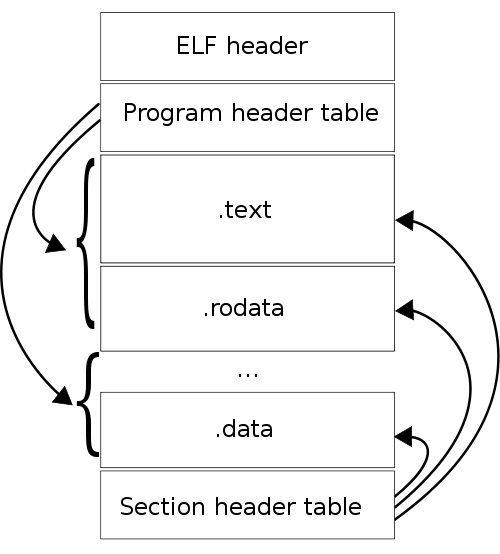
\includegraphics[keepaspectratio=true,width=\framewidth]{Elf-layout.png}
\end{frame}

\begin{frame}{Further Reading}
  \begin{itemize}
    \item
      https://en.wikipedia.org/wiki/Executable\_and\_linkable\_Format
    \item https://en.wikipedia.org/wiki/Objdump
    \item https://en.wikipedia.org/wiki/Reverse\_engineering
    \item https://www.eff.org/issues/coders
  \end{itemize}
\end{frame}

\end{document}
